\section{Experiments}
\label{sec:experiments}

\begin{table*}[t]
\caption{\textbf{Comparison on all 18 scenes of three OLAT benchmarks} (5,691 test images, identical targets, original test calibration, no test-time fitting; best in \textbf{bold}, second \underline{underlined}). Iterations: RNG 30k+70k, OLAT-GS 30k+30k, GS$^3$ 100k, SSD-GS 100k (60k on SSS), LiSA 38k.}
\label{tab:main}
\centering\small
\setlength{\tabcolsep}{4.2pt}
\begin{tabular}{@{}l ccc ccc ccc ccc@{}}
\toprule
 & \multicolumn{3}{c}{NRHints, real (7)} & \multicolumn{3}{c}{GS$^3$, synthetic (6)} & \multicolumn{3}{c}{SSS-GS, synthetic (5)} & \multicolumn{3}{c}{All scenes (18)} \\
\cmidrule(lr){2-4}\cmidrule(lr){5-7}\cmidrule(lr){8-10}\cmidrule(l){11-13}
Method & PSNR$\uparrow$ & SSIM$\uparrow$ & LPIPS$\downarrow$ & PSNR$\uparrow$ & SSIM$\uparrow$ & LPIPS$\downarrow$ & PSNR$\uparrow$ & SSIM$\uparrow$ & LPIPS$\downarrow$ & PSNR$\uparrow$ & SSIM$\uparrow$ & LPIPS$\downarrow$ \\
\midrule
RNG~\cite{fan2025rng} & 20.94 & .828 & .203 & 22.14 & .895 & .132 & 37.10 & .983 & .028 & 25.83 & .893 & .131 \\
OLAT-GS~\cite{kuang2024olat} & 27.26 & \underline{.886} & \underline{.114} & 27.11 & .940 & .079 & \textbf{40.74} & \textbf{.990} & \textbf{.016} & 30.95 & .933 & .075 \\
GS$^3$~\cite{bi2024gs3} & \underline{27.28} & .884 & .116 & \underline{31.97} & \underline{.967} & \underline{.049} & 36.81 & .983 & .028 & 31.49 & \underline{.939} & .069 \\
SSD-GS~\cite{zheng2026ssdgs} & 27.20 & .882 & .117 & 31.53 & .965 & .050 & 37.79 & \underline{.986} & \underline{.023} & \underline{31.59} & \underline{.939} & \underline{.068} \\
\midrule
\textbf{LiSA (ours)} & \textbf{29.28} & \textbf{.909} & \textbf{.100} & \textbf{32.40} & \textbf{.970} & \textbf{.038} & \underline{40.63} & \textbf{.990} & \textbf{.016} & \textbf{33.47} & \textbf{.952} & \textbf{.056} \\
\bottomrule
\end{tabular}
\end{table*}


\subsection{Setup}
\label{sec:setup}
\paragraph{Data.}
We use every scene of three public OLAT benchmarks: the seven real captures of NRHints~\cite{zeng2023nrhints} (522--1500 training and 66--200 test images each), the six HDR synthetic scenes of \gsthree~\cite{bi2024gs3} (2000/400), and the five subsurface-scattering scenes of SSS-GS~\cite{dihlmann2024sss} (500/500).
We keep each benchmark's conventions (512\,px images, 256\,px for SSS-GS; white background and $\gamma=2.2$ display for HDR) and use all official training and all 5,691 test images.

\paragraph{Baselines.}
We compare with the four recent Gaussian methods that train per scene from point-light captures and provide code, \gsthree~\cite{bi2024gs3}, SSD-GS~\cite{zheng2026ssdgs}, OLAT Gaussians (OLAT-GS)~\cite{kuang2024olat} and RNG~\cite{fan2025rng}, retrained with their released code and default schedules (60k--100k iterations; ours: 38k).
All use the foreground masks (to composite targets; OLAT-GS also for its surface stage, \ours also for an opacity loss); \gsthree, SSD-GS and OLAT-GS refine training poses on real captures, and no method fits test cameras or lights.
RNG and OLAT-GS fall below 21\,dB on several scenes (\eg, Drums, Lego), possibly because these violate their assumptions (black-background LDR data; a proxy surface); we report these runs unchanged.
\todo{[E5, E6] Add SSS-GS~\cite{dihlmann2024sss} once a stable reproduction exists (our runs diverged on three of five scenes) and reproduce one published configuration per baseline.}

\paragraph{Metrics and protocol.}
We report PSNR, SSIM~\cite{wang2004image} and VGG-LPIPS~\cite{zhang2018unreasonable} on full images, averaged over the test views of each scene and then over scenes, and test per-scene differences with a Wilcoxon signed-rank test.
All predictions are scored against one common set of 8-bit targets (changing the baselines' averages by at most 0.005\,dB), and foreground-masked PSNR preserves the ranking within every benchmark (supplement); main results use one run per method and scene, ablations three seeds.
Earlier versions of \ours were evaluated on these benchmarks during development (supplement); the final configuration was selected on views held out from the training sets and is shared by all scenes.

\subsection{Comparison with the state of the art}
\label{sec:exp_main}
\ours has the best average PSNR, SSIM and LPIPS over the 18 scenes (\cref{tab:main}), 1.89\,dB ahead of SSD-GS, and its per-scene advantage over every baseline is significant ($p\le0.016$).
No baseline is consistent across benchmarks: OLAT-GS is best on SSS-GS but trails \ours by 5.3\,dB on the \gsthree scenes, and \gsthree is second on its own scenes but last on SSS-GS.
\ours is the only method among the top two on every benchmark and has the best LPIPS on all three.
The margin is concentrated, however: three real captures contribute 46\% of it, \ours and \gsthree each win three of the six \gsthree scenes in PSNR (\ours wins five in LPIPS), and on the 11 synthetic scenes, where calibration is exact, \ours leads SSD-GS by 1.77\,dB ($p=0.014$) but not OLAT-GS significantly ($p=0.12$).

The largest gains occur where moving cast shadows and light crossing translucent objects dominate: 1.90\,dB on Hotdog and 1.91\,dB on Translucent over the best baseline.
In \cref{fig:comparison}, the shadows of the vase handle and the hot dogs fall across large floor and plate Gaussians; per-primitive visibility fragments them, while pixel receivers reading the atlas reproduce their outlines.
\ours trails on Drums ($-1.09$\,dB) and AnisoMetal ($-0.85$\,dB), whose thin or anisotropic highlights our isotropic lobes miss.

On real captures \ours leads by 2.0\,dB on average, entirely due to Cat, Fish and Pixiu; on the other four it trails \gsthree by 0.3\,dB.
Fixed-calibration scores here depend on registration as well as appearance: the official poses carry small errors, and refining training poses without anchoring the reconstruction can shift it relative to the test cameras, which our gauge-constrained refinement (\cref{sec:implementation}) avoids by construction.
Aligning every test rendering by its best 2D shift (supplement) shows the effect: the baselines need 4.0--4.6\,px against 1.7\,px for \ours, and the lead of \ours shrinks to 0.7\,dB, staying large on Cat and Pixiu but vanishing on Fish.
\torun{E2: \ours without pose refinement and a rotation-only test-pose alignment for all methods.}

\begin{figure*}[t]
\centering
\setlength{\tabcolsep}{0.8pt}
\renewcommand{\arraystretch}{0.5}
\newcommand{\cw}{0.131\textwidth}
\begin{tabular}{@{}ccccccc@{}}
\small Test view & \small Ground truth & \small \ours (ours) & \small SSD-GS & \small \gsthree & \small OLAT-GS & \small RNG \\[2pt]
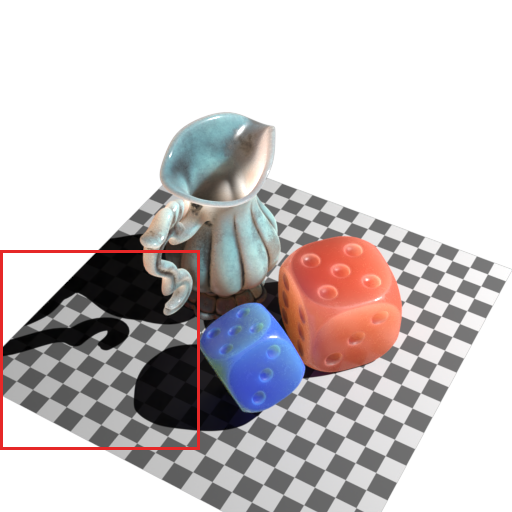
\includegraphics[width=\cw]{figures/comparison/translucent/full.png} & 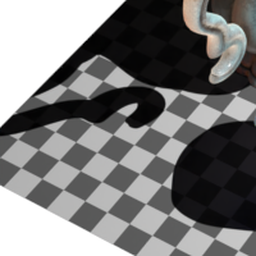
\includegraphics[width=\cw]{figures/comparison/translucent/GT.png} & 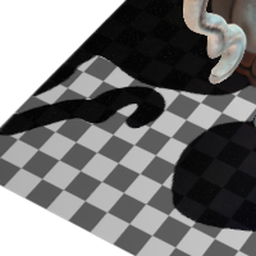
\includegraphics[width=\cw]{figures/comparison/translucent/LiSA-staged.png} & 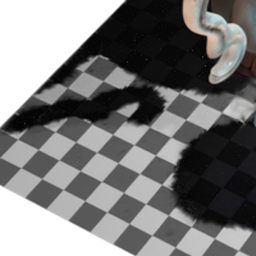
\includegraphics[width=\cw]{figures/comparison/translucent/SSD-GS.png} & 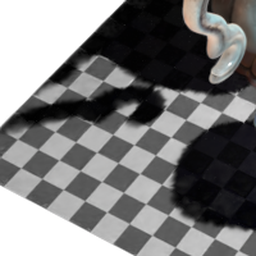
\includegraphics[width=\cw]{figures/comparison/translucent/GS3.png} & 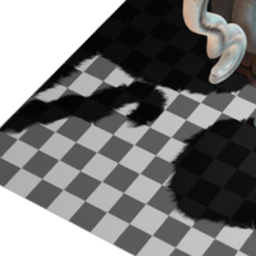
\includegraphics[width=\cw]{figures/comparison/translucent/OLAT-Gaussians.png} & 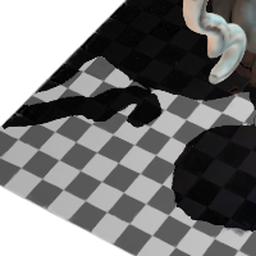
\includegraphics[width=\cw]{figures/comparison/translucent/RNG.png} \\
\footnotesize Translucent & \footnotesize PSNR & \footnotesize \textbf{34.36} & \footnotesize 32.28 & \footnotesize 32.58 & \footnotesize 29.93 & \footnotesize 27.92 \\[3pt]
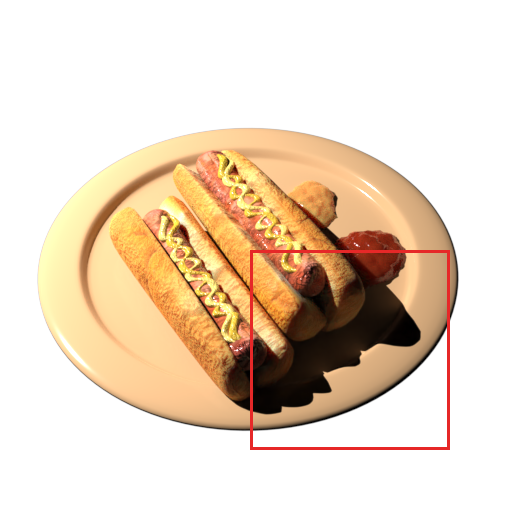
\includegraphics[width=\cw]{figures/comparison/hotdog/full.png} & 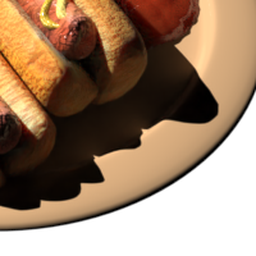
\includegraphics[width=\cw]{figures/comparison/hotdog/GT.png} & 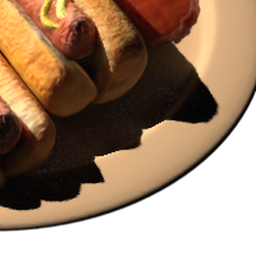
\includegraphics[width=\cw]{figures/comparison/hotdog/LiSA-staged.png} & 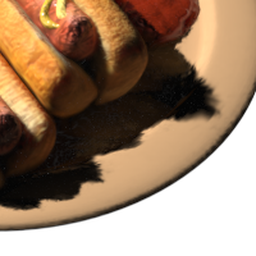
\includegraphics[width=\cw]{figures/comparison/hotdog/SSD-GS.png} & 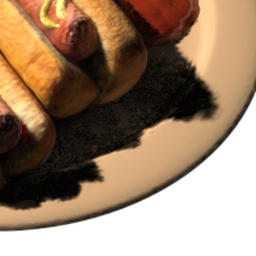
\includegraphics[width=\cw]{figures/comparison/hotdog/GS3.png} & 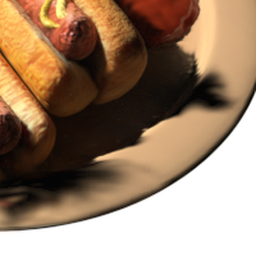
\includegraphics[width=\cw]{figures/comparison/hotdog/OLAT-Gaussians.png} & 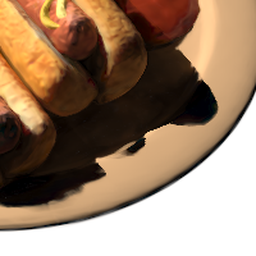
\includegraphics[width=\cw]{figures/comparison/hotdog/RNG.png} \\
\footnotesize Hotdog & \footnotesize PSNR & \footnotesize \textbf{33.97} & \footnotesize 31.93 & \footnotesize 32.08 & \footnotesize 26.85 & \footnotesize 28.49 \\[3pt]
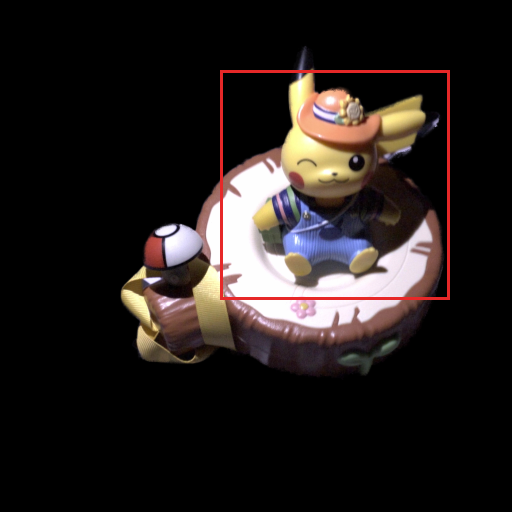
\includegraphics[width=\cw]{figures/comparison/pikachu/full.png} & 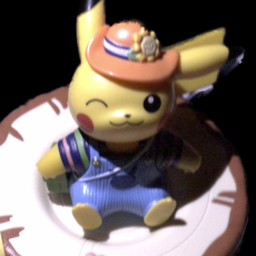
\includegraphics[width=\cw]{figures/comparison/pikachu/GT.png} & 
\includegraphics[width=\cw]{figures/comparison/pikachu/LiSA-staged.png} & 
\includegraphics[width=\cw]{figures/comparison/pikachu/SSD-GS.png} & 
\includegraphics[width=\cw]{figures/comparison/pikachu/GS3.png} & 
\includegraphics[width=\cw]{figures/comparison/pikachu/OLAT-Gaussians.png} & 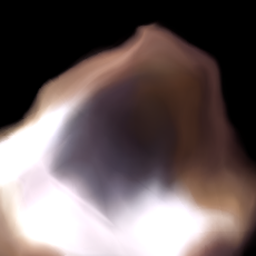
\includegraphics[width=\cw]{figures/comparison/pikachu/RNG.png} \\
\footnotesize Pikachu (real) & \footnotesize PSNR & \footnotesize 30.44 & \footnotesize 29.58 & \footnotesize \textbf{30.71} & \footnotesize 29.46 & \footnotesize 16.31 \\[3pt]
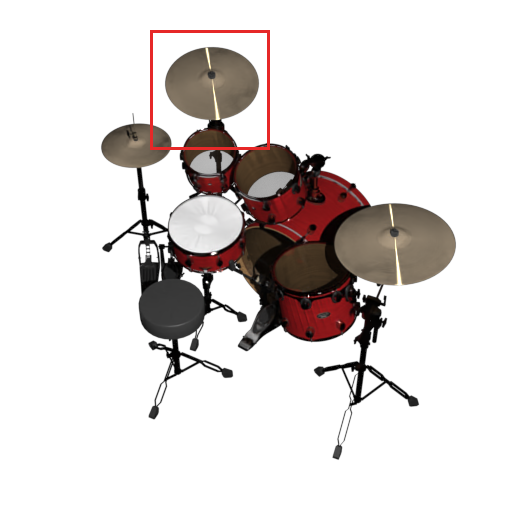
\includegraphics[width=\cw]{figures/comparison/fail_drums/full.png} & 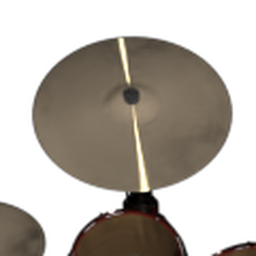
\includegraphics[width=\cw]{figures/comparison/fail_drums/GT.png} & 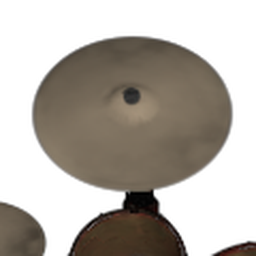
\includegraphics[width=\cw]{figures/comparison/fail_drums/LiSA-staged.png} & 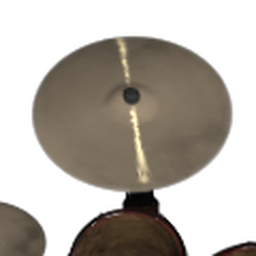
\includegraphics[width=\cw]{figures/comparison/fail_drums/SSD-GS.png} & 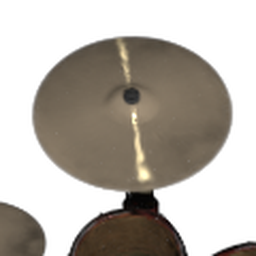
\includegraphics[width=\cw]{figures/comparison/fail_drums/GS3.png} & 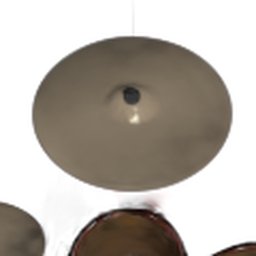
\includegraphics[width=\cw]{figures/comparison/fail_drums/OLAT-Gaussians.png} & 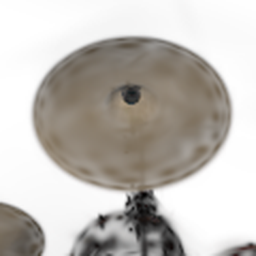
\includegraphics[width=\cw]{figures/comparison/fail_drums/RNG.png} \\
\footnotesize Drums & \footnotesize PSNR & \footnotesize 30.90 & \footnotesize 31.32 & \footnotesize \textbf{31.93} & \footnotesize 22.23 & \footnotesize 16.23 \\[3pt]
\end{tabular}
\caption{\textbf{Qualitative comparison} on test views (crops of the boxed region; PSNR of the full view), each at the median of \ours's per-view margin over the best baseline in its scene. Rows: the two \gsthree scenes dominated by cast shadows, a real capture on which the methods are close, and the synthetic scene where we trail most. Per-primitive shadows of SSD-GS and \gsthree fragment the moving shadows of the vase handle and the hot dogs, which pixel receivers reading the atlas reproduce; \ours misses the thin streak on the Drums cymbal. More scenes, including Fish, are in the supplement.}
\label{fig:comparison}
\end{figure*}


\subsection{What the atlas contributes}
\label{sec:exp_atlas}
\Cref{tab:ablation} ablates the atlas on a panel of five scenes covering opaque, metallic, furry, translucent and subsurface-scattering materials, including three of the scenes where we trail most; the full model varies by 0.11\,dB across seeds.
Using only the finest atlas level costs 0.44\,dB and replacing the learned visibility by the moment test of \cref{eq:moment} costs 0.24\,dB; these single-seed differences only suggest that both matter, and the panel does not yet compare atlas visibility with per-primitive visibility or a plain shadow map at the same receivers, which E3 does.

\begin{table}[t]
\caption{\textbf{Ablation of the atlas} on five scenes (Drums, AnisoMetal, Translucent, FurScene, Soap), scene-averaged. For rows with three seeds we report the mean over seeds and the standard deviation of PSNR; single-seed rows compare to the seed-0 full model (31.53\,dB). $^\dagger$Capacity-matched MLP (49.1k vs.\ 49.6k parameters) that reads the receiver's code, position and light/view directions but not the atlas; shadows still come from the atlas.}
\label{tab:ablation}
\centering\small
\setlength{\tabcolsep}{3.5pt}
\begin{tabular}{@{}lcccc@{}}
\toprule
Variant & Seeds & PSNR$\uparrow$ & SSIM$\uparrow$ & LPIPS$\downarrow$ \\
\midrule
Full model & 3 & 31.51{\tiny$\pm$0.11} & .954 & .047 \\
w/o transfer term & 3 & 30.15{\tiny$\pm$0.11} & .948 & .055 \\
transfer $\rightarrow$ local residual$^\dagger$ & 3 & 31.54{\tiny$\pm$0.03} & .954 & .047 \\
single atlas level ($K{=}1$) & 1 & 31.09 & .952 & .049 \\
moment test only ($g\equiv 0$) & 1 & 31.29 & .952 & .048 \\
per-Gaussian visibility$^\ddagger$ & 3 & \TBD & \TBD & \TBD \\
hard shadow map$^\ddagger$ & 3 & \TBD & \TBD & \TBD \\
\bottomrule
\end{tabular}
\\[2pt]{\footnotesize$^\ddagger$\torun{E3 (same receivers; atlas kept for transfer); also three seeds for the single-seed rows.}}
\end{table}

\begin{table}[t]
\caption{\textbf{Where the transfer term matters.} Per-scene PSNR differences (mean$\pm$std of paired differences over three seeds) of the full model against removing the transfer term and against the capacity-matched local residual, and the share of linear radiance the full model routes through the transfer term (mean over 8 test views).}
\label{tab:paired}
\centering\small
\setlength{\tabcolsep}{4pt}
\begin{tabular}{@{}lccc@{}}
\toprule
Scene & vs.\ w/o transfer & vs.\ local residual & Transfer share \\
\midrule
Drums & $+0.10${\tiny$\pm$0.02} & $-0.09${\tiny$\pm$0.02} & 6\% \\
FurScene & $+0.02${\tiny$\pm$0.03} & $+0.02${\tiny$\pm$0.02} & 7\% \\
AnisoMetal & $+1.42${\tiny$\pm$0.69} & $-0.18${\tiny$\pm$0.75} & 7\% \\
Translucent & $+2.29${\tiny$\pm$0.23} & $+0.41${\tiny$\pm$0.26} & 17\% \\
Soap & $+2.99${\tiny$\pm$0.30} & $-0.29${\tiny$\pm$0.11} & 58\% \\
\bottomrule
\end{tabular}
\end{table}


Removing the transfer term costs 1.37\,dB and raises LPIPS from 0.047 to 0.055, on all three seeds, and the cost follows the material (\cref{tab:paired}): it is negligible on Drums and FurScene, 1.42\,dB on AnisoMetal, and 2.29 and 2.99\,dB on Translucent and Soap.
The model routes 6--7\% of its linear radiance through the transfer term on the first three scenes but 17\% on Translucent and 58\% on Soap (over all 18 scenes, 6--9\% on opaque synthetic objects and 20--58\% on subsurface-scattering ones), a learned allocation rather than a physical decomposition.

To separate the atlas from the extra radiance path, we replace the atlas transfer by a capacity-matched MLP that reads the receiver's code, position and light and view directions but not the atlas, keeping the atlas shadows.
This local residual is on par with the full model on average (31.54 vs.\ 31.51\,dB), so on most of these materials the transfer term mainly supplies an unshadowed, nonnegative radiance path that a local network provides equally well.
The atlas is ahead only on Translucent, where light visibly crosses the object before reaching the visible surface ($+0.41\pm0.26$\,dB, positive for all three seeds but not significant), while the local residual is ahead on Soap ($-0.29\pm0.11$\,dB) and marginally on Drums; on AnisoMetal the full model is also less stable across seeds (26.4--27.9\,dB).
We therefore do not attribute our overall margin to the transfer term, and hypothesize that it stems from the light-space visibility and the optimization schedule, which E3 and E4 test.
The light-relative design should matter most under light extrapolation, which the benchmarks do not probe: their test lights lie a median of $1.1^\circ$ from the nearest training light.
\torun{E1 (\cref{tab:holdout}): three seeds on the ablation panel; to be verified, not assumed: the atlas degrades less than the local residual.}

\begin{table}[t]
\caption{\textbf{Held-out light directions} (\torun{E1}). Mean PSNR over the five ablation scenes on the official test views and on training-split views whose lights fall in held-out 30$^\circ$ angular groups, after retraining every method without those views. $^\dagger$Three seeds.}
\label{tab:holdout}
\centering\small
\begin{tabular}{@{}lccc@{}}
\toprule
Method & Official test & Held-out lights & Drop \\
\midrule
\gsthree & 31.25 & \TBD & \TBD \\
SSD-GS & 31.01 & \TBD & \TBD \\
OLAT-GS & 28.67 & \TBD & \TBD \\
\ours, local residual$^\dagger$ & 31.54 & \TBD & \TBD \\
\ours$^\dagger$ & 31.51 & \TBD & \TBD \\
\bottomrule
\end{tabular}
\end{table}

\begin{figure}[t]
\centering
\setlength{\tabcolsep}{0.8pt}
\renewcommand{\arraystretch}{0.5}
\newcommand{\lw}{0.322\linewidth}
\begin{tabular}{@{}ccc@{}}
\small display-domain loss & \small radiometric schedule & \small ground truth \\[2pt]
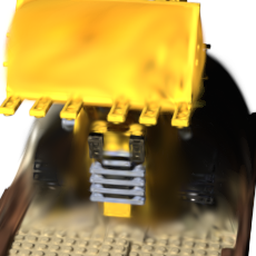
\includegraphics[width=\lw]{figures/loss_domain/lego/control_crop.png} & 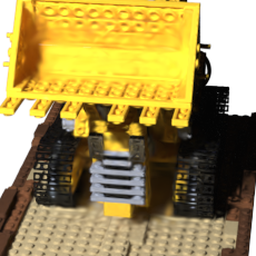
\includegraphics[width=\lw]{figures/loss_domain/lego/ours_crop.png} & 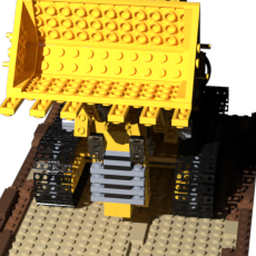
\includegraphics[width=\lw]{figures/loss_domain/lego/gt_crop.png} \\
\footnotesize 23.02\,dB & \footnotesize \textbf{30.25\,dB} & \footnotesize Lego \\[3pt]
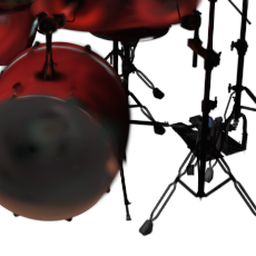
\includegraphics[width=\lw]{figures/loss_domain/drums/control_crop.png} & 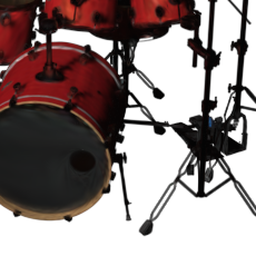
\includegraphics[width=\lw]{figures/loss_domain/drums/ours_crop.png} & 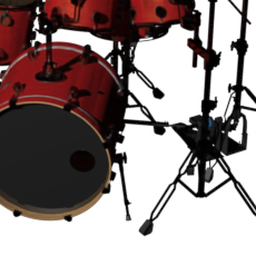
\includegraphics[width=\lw]{figures/loss_domain/drums/gt_crop.png} \\
\footnotesize 24.10\,dB & \footnotesize \textbf{30.10\,dB} & \footnotesize Drums \\[3pt]
\end{tabular}
\caption{\textbf{Loss domain and geometry.} Two runs that share initialization, schedule, random state and every other setting, differing only in whether the loss is computed on display-encoded or (after the annealed warm-up) linear radiance; 16k iterations, PSNR over 200 held-out training views. All 200 views improve on both scenes.}
\label{fig:loss_domain}
\end{figure}


\subsection{What the optimization contributes}
\label{sec:exp_optimization}
\paragraph{Loss domain.}
On Lego and Drums, where our first runs failed, two 16k-iteration runs share the initialization, warm-up stage, schedule and random states, and differ only in the loss: the control uses display-encoded radiance throughout, ours follows stages I and II.
On 200 views held out from the training set, the display-domain geometry collapses (\cref{fig:loss_domain}), while the radiometric schedule raises PSNR from 23.02 to 30.25\,dB on Lego and from 24.10 to 30.10\,dB on Drums (LPIPS 0.122$\to$0.057 and 0.060$\to$0.034), improving every view by a median of 7.2 and 6.0\,dB.
The study covers two HDR scenes, one seed and 16k iterations; on real and SSS-GS scenes, an earlier display-domain version of \ours, which also differs otherwise, scores 0.2--0.4\,dB higher (supplement).
\torun{E4: on the ablation panel, three seeds: (a) display-domain loss throughout, (b) no warm-up, (c) pixel receivers in stage II, (d) no stage III, (e) an offset inside $\Gamma$.}

\paragraph{Receivers and refinement.}
On frozen 30k geometry of Lego, Drums and Soap (Tab.~S6 in the supplement), refining in the display domain instead of linear radiance improves all three metrics for both kinds of receivers (PSNR $+0.20$\,dB for Gaussians and $+0.28$\,dB for pixels).
Pixel receivers give the best SSIM and LPIPS (0.976 and 0.029) and Gaussian receivers a 0.19\,dB higher PSNR; we keep pixels for their perceptual quality.

\subsection{Cost}
\label{sec:exp_cost}
Profiled on an otherwise idle GPU on Drums, FurScene and Soap (Tab.~S5 in the supplement), \ours trains 1.6--5.5 times faster than \gsthree and SSD-GS and uses 228k Gaussians on Drums against about 550k for both; over all 18 scenes, timed under less uniform conditions, its mean training time is 21 minutes against 55--107 for the baselines.
The light pass keeps rendering interactive at 63--104 frames per second with a new light every frame, but makes \ours slower than \gsthree and SSD-GS on small scenes.

\subsection{Limitations}
\label{sec:limitations}
Isotropic lobes miss brushed metal and thin streaks: on Drums, 0.27\% of the pixels, flagged as narrow highlights in the ground truth, carry 72\% of our excess squared error relative to \gsthree.
The moment test is a weak prior for mixed footprints and center depths misplace large oblique Gaussians, for which Chebyshev or four-moment tests~\cite{donnelly2006variance,peters2015moment} and intersection depths are natural fixes.
One perspective atlas assumes the light lies outside the object, the transfer term ignores the solid-angle factor and the entry-point falloff, and light reaching a receiver only through regions the light cannot see is beyond one light-space gather.
